\chapter{Architektura systemów operacyjnych w zastosowaniach wbudowanych}\label{}
Projektowanie złożonych systemów komputerowych, zwłaszcza takich jak rozwiązania bazujące na implementacji algorytmów przetwarzania sygnałów w rygorze czasu rzeczywistego przy jednocześnie ograniczonych zasobach sprzętowych, jest zadaniem, które wymaga wielu przemyślanych decyzji przy doborze architektury tworzonego systemu.

Wybór odpowiedniej platformy programowej jest jedną z kluczowych decyzji projektowych. Projektant systemu wbudowanego staje wówczas często przed wyborem między podejściem bezsystemowym, zapewniającym pełną kontrolę nad sprzętem, a zastosowaniem systemu operacyjnego, który wprowadza warstwę abstrakcji kosztem częściowej utraty determinizmu czasowego oraz zwiększenia zużycia fizycznych zasobów systemu \cite{Tanenbaum}. Decyzja ta ma bezpośredni wpływ na poprawność systemu, nie tylko z uwagi na osiąganą wydajność obliczeniową, ale również poprzez bezpieczeństwo i stabilność systemu.
W celu zwiększenia jakości projektowanego systemu inżynier oprogramowania powinien posiadać niezbędną wiedzę teoretyczną z zakresu działania systemów operacyjnych, aby zagwarantować tworzenie możliwie wydajnych i niezawodnych systemów komputerowych.

Celem prezentowanego rozdziału jest usystematyzowanie wiedzy niezbędnej do zrozumienia, w jaki sposób architektura stosowanego systemu operacyjnego wpływa na wydajność uruchamianych na nim programów. Rozważania rozpoczynają się od przedstawienia warstwowego modelu systemów operacyjnych oraz kluczowych mechanizmów jądra, takich jak tryby pracy procesora, procesy, wątki, szeregowanie zadań, pamięć wirtualna oraz synchronizacja współbieżnych operacji. Na tej podstawie omówiony zostaje podział systemów wbudowanych czasu rzeczywistego, a także dwa podstawowe modele budowy jądra: architektura monolityczna oraz mikrojądrowa. Ostatnia część rozdziału zawiera studium przypadku systemu operacyjnego Linux, w którym w skrócony sposób starano się przedstawić niezbędne szczegóły implementacji mechanizmów systemowych.

\section{Rola systemów operacyjnych w systemach wbudowanych}

%Tutaj dajemy zdanie wprowadzające, ze przy projektowaniu systemow wbudowanych mozna podejsc roznie do tematu
Podczas projektowania systemu wbudowanego, włączając w to system wbudowany czasu rzeczywistego, projektant staje przed wyborem jednego z dwóch podstawowych podejść do organizacji i kontroli całego środowiska. 
Pierwszym z nich jest \textbf{podejście bezsystemowe}  (ang. \textit{bare-metal}), w którym całe oprogramowanie funkcjonuje bez żadnej warstwy pośredniej, 
mając bezpośredni i wyłączny dostęp do fizycznych układów procesora oraz peryferiów. 
Choć pozwala to na pełną kontrolę nad sprzętem i minimalne narzuty czasowe, to drastycznie ogranicza skalowalność każda zmiana komponentu 
lub rozbudowa funkcji wymusza wówczas głęboką modyfikację struktury całego kodu.

Alternatywą jest zastosowanie \textbf{systemu operacyjnego}, który możemy zdefiniować jako podstawowe oprogramowanie pośredniczące między sprzętem komputerowym a użytkownikiem, 
którego głównym zadaniem jest zarządzanie i przydzielanie zasobów sprzętowych oraz tworzenie środowiska pozwalającego na wykonywanie programów zaimplementowanych przez jego użytkownika \cite{Abraham_Silberschatz}.

Jak wynika z przytoczonej definicji, stosowanie systemu operacyjnego pomaga rozwiązywać niektóre problemy napotykane przy stosowaniu podejścia bezsystemowego. 
Dzieje się tak poprzez całościowe odizolowanie warstwy programowej od fizycznych struktur sprzętu.
System operacyjny działa jako nadrzędny pośrednik, przejmując na siebie zadanie nadzorowania środowiska wykonawczego i separując logikę działania
od konkretnej platformy sprzętowej. 

Aby w pełni zrozumieć, jak system operacyjny realizuje te zadania w środowisku wbudowanym, konieczne jest przyjrzenie się jego wewnętrznej architekturze.
 W dalszych sekcjach zostaną szczegółowo omówione kluczowe mechanizmy oraz podstawowa struktura ogólnych systemów operacyjnych.

\subsection{Model warstwowy systemów operacyjnych}


W inżynieri oprogramowania istotną rolę odgrywa koncepcja \textbf{abstrakcji}, polegająca na  celowym ukryciu szczegółów implementacji danej funkcjonalności oprogramowania, przed jej potencjalnym użytkownikiem \cite{Tanenbaum}.
Podejście to opiera się na założeniu, że należy dostarczyć gotowe funkcjonalność  wraz z odpowiednią dokumentacją opisującą sposób jej wykorzystania, zamiast wymagać od użytkownika zrozumienia wewnętrznych mechanizmów działania wytworzonego modułu.

Taka praktyka w sposób znaczący podnosi wygodę wytwarzania nowych elementów systemu, umożliwia zrównoleglenie wytwarzania oprogramowania oraz pozwala na większą specjalizacje jej producentów. 
W celu realizacji komunikacji między kolejnymi modułami systemu stosuj się takie narzędzia jak \textbf{interfejsy programistyczne} (ang. \textit{Application Programming Interface}, skrót \textbf{API}), czyli zbiór ściśle określonych reguł i sposobów komunikacji, które umożliwają komunikację między różnymi warstwami oprogramowania.
Narzędzie to jest niezbędne, aby w sposób przewidywalny i bezpieczny przekazywać danę lub sterowanie, między różnymi elemenetami systemu.

Pojęcie abstrakcji jest kluczowe dla zrozumienia architektury współczesnych systemów operacyjnych. 
W literaturze spotyka się różne podejścia do klasyfikacji poziomów systemu komputerowego \cite{Tanenbaum, Abraham_Silberschatz}, jednak ich cechą 
wspólną jest wyraźne odseparowanie zasobów fizycznych od uruchamianego na nich oprogramowania. 
Na potrzeby niniejszej pracy przyjęto strukturę opartą na propozycji przedstawionej w \cite{Abraham_Silberschatz}, którą w graficzny sposób zaprezentowano na rysunku \ref{fig:rysunek1}.

\begin{figure}[h]
    \centering
    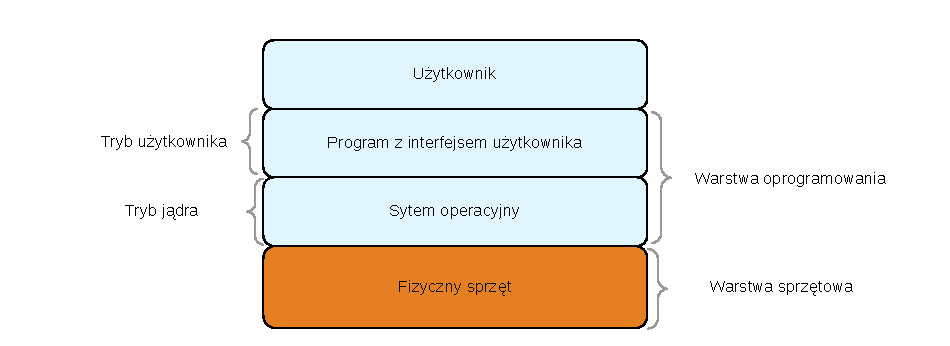
\includegraphics[width=0.8\textwidth]{img/Rysunek1.pdf}
    \caption{Warstwowy model systemu komputerowego}
    \label{fig:rysunek1}
\end{figure}

Jak pokazano na schemacie, najniższy poziom stanowi warstwa sprzętowa, do której zalicza się wszystkie fizyczne komponenty urządzenia,
takie jak \textbf{jednostka centralna} (ang. \textit{Central Processing Unit}, CPU), \textbf{pamięć} oraz \textbf{urządzenia wejścia-wyjścia} (ang. \textit{Input/Output Devices}, I/O). 
Ponad nią znajduje się warstwa oprogramowania, na którą składa się zarówno system operacyjny, jak i programy użytkownika. 
Choć oba te elementy należą do tej samej warstwy, funkcjonują one na innych zasadach. Odróżnia je praca w różnych trybach procesora, różniących się poziomem uprawnień oraz zakresem dostępu do fizycznych urządzeń.
Tryby te nazywają się odpowiednio \textbf{trybem jądra} (ang. \textit{kernel mode}), dla systemu operacyjnego, oraz \textbf{trybem użytkownika} (ang. \textit{user mode}), dla aplikacji użytkownika. 
Szczegółowa omównienie przytoczonych trybów oraz mechanizmów ich przełączania zostanie omówiona w dalszych częściach tego rozdziału.

Warto przy tym podkreślić, że w przytoczonej pozycji literatury \cite{Abraham_Silberschatz} jako integralny komponent struktury systemu komputegowego uwzględnia się jego użytkownika. 
Zabieg ten ma na celu jednoznaczne wskazanie, że przy projektowaniu dowolnego systemu komputerowego należy zawsze pamiętać o jego ostatecznym przeznaczeniu oraz o użytkowniku końcowym.

W modelu warstwowym architektury komputerowej system operacyjny pełni szczególną rolę, zarządzając granicą między aplikacjami a warstwą fizyczną. W celu zapewnienia poprawnego i przewidywalnego działania systemu wprowadza poziomy abstrakcji, które są niezbędne z kilku istotnych powodów:

\begin{enumerate}
\item \textbf{Konieczność zapewnienia bezpieczeństwa } - Współczesne systemy operacyjne charakteryzują się ogromną złożonością, a ich kod źródłowy sięga kilkudziesięciu milionów linii \cite{Tanenbaum}.
 Izolacja poszczególnych poziomów wprowadza wyraźną hierarchię uprawnień. Dzięki temu błąd powstały w kodzie aplikacyjnym pozostaje odizolowany i nie wpływa bezpośrednio na stabilność pozostałych funkcjonalności systemowych ani na pracę samego sprzętu.
\item \textbf{Zapewnienie przenoszalności oprogramowania} - Zastosowanie warstw pośrednich sprawia, że oprogramowanie nie jest bezpośrednio uzależnione od konkretnych urządzeń fizycznych. Pozwala to na uruchamianie tych samych programów na różnorodnych platformach sprzętowych,
 umożliwiając przy tym niezależny rozwój warstwy aplikacyjnej i sprzętowej.
\item \textbf{Umożliwienie korzystania z narzędzi wysokiego poziomu} - Ukrycie technicznych szczegółów pracy ze sterownikami lub rejestrami pozwala na tworzenie kodu w językach wysokiego poziomu. Programista może skupić się na logice i strukturze zgodnej ze sposobem myślenia człowieka, zamiast na bezpośredniej, niskopoziomowej obsłudze układów elektronicznych.
\end{enumerate}
\section{Kluczowe abstrakcje i mechanizmy stosowane w systemach operacyjnych}
Pomimo dużej różnorodności współczesnych systemów operacyjnych, ich architektura opiera się na spójnym zestawie uniwersalnych abstrakcji i mechanizmów. Od strony koncepcyjnej rozwiązania te wprowadzają ład w złożonym środowisku sprzętowym, przybliżając sposób funkcjonowania komputera do logiki myślenia i pracy człowieka. 

Koncepcje opisane w prezentowanej sekcji pozwalają na stworzenie przejrzystego i uporządkowanego modelu zarządzania zasobami w systemie operacyjnym. 
Zrozumienie tych bazowych koncepcji jest kluczowe dla analizy wydajności, ponieważ to one determinują sposób, w jaki program aplikacji, stworznej przez użytkownika, jest uruchamiany i wykonywany na fizycznym sprzęcie.

Na potrzeby niniejszej pracy konieczne jest przedstawienie następujących pojęć i mechanimów:
\begin{itemize}
    \item  \textbf{Tryby pracy procesora}
    \item \textbf{Proces}
    \item  \textbf{Wątek}
    \item \textbf{Szeregowanie zadań}
    \item \textbf{Pamięć wirtualna}
    \item \textbf{Mechanizmy synchronizacji i współbieżności}
\end{itemize}
\subsection{Tryby pracy procesora}
Współczesne komputery realizują ochronę zasobów poprzez tryby pracy procesora \cite{Abraham_Silberschatz}, z których kluczowe to \textbf{tryb użytkownika} (ang. user mode) oraz \textbf{tryb jądra} (ang. kernel mode). Aplikacje użytkownika funkcjonują w trybie użytkownika, nieuprzywilejowanym, co uniemożliwia im między innymi, bezpośredni dostęp do urządzeń peryferyjnych oraz fizycznej pamięci.

Wszelkie operacje wymagające kontroli nad sprzętem realizowane są za pośrednictwem \textbf{wywołań systemowych} \cite{Abraham_Silberschatz} (ang. system calls), które przełączają procesor w uprzywilejowany tryb jądra.

\subsection{Procesy}
\textbf{Proces} (ang. \textit{process}) można rozumieć jako wykonujący się program komputerowy \cite{Abraham_Silberschatz}.Jego kluczową cechą jest przydzielona, odizolowana od innych procesów wirtualna \textbf{przestrzeń adresowa}
Jej wprowadzenie ma zagwarantować bezpieczeństwo – błąd w obrębie jednego procesu nie wpływa bezpośrednio na stabilność procesów systemowych i innych procesów użytkownika.  

Współczesne systemy komputerowe składają się z licznych komponentów i aplikacji, co sprawia, że na wspólnych, fizycznych zasobach sprzętowych funkcjonuje jednocześnie wiele procesów. 
Ze względu na to, że pojedynczy rdzeń procesora może w danej chwili realizować tylko jedno zadanie, system operacyjny stosuje przełączanie kontekstu, cyklicznie przydzielając czas procesora poszczególnym procesom.
Ponieważ każdy proces operuje w odrębnej przestrzeni adresowej, zmiana ta wymaga przeładowania pamięci operacyjnej. 
W efekcie przełączanie kontekstu między procesami jest operacją stosunkowo czasochłonną i wiąże się z zauważalnym opóźnieniem, które można nazywać też \textbf{narzutem systemu operacyjnego} \cite{Tanenbaum}.

\subsection{Wątki}
\textbf{Wątek} (ang. \textit{thread}) stanowi wyodrębnioną jednostkę wykonawczą (ciąg instrukcji) uruchamianą na procesorze, funkcjonującą w obrębie konkretnego procesie \cite{Tanenbaum}. 

W ramach jednego procesu może działać wiele wątków wykonujących się we wspólnej przestrzeni adresowej. Wątki należące do tego samego procesu współdzielą ze sobą zasoby systemowe (m.in. przestrzeń adresową, zmienne globalne czy otwarte pliki), jednak każdy z nich posiada własny, prywatny kontekst wykonania \cite{Tanenbaum}, na który składają się:
\begin{itemize}
    \item \textbf{Licznik instrukcji} (ang. \textit{Program Counter}),
    \item \textbf{Zestaw rejestrów procesora},
    \item \textbf{Prywatny stos} (przechowujący zmienne lokalne oraz historię wywołań funkcji),
    \item \textbf{Stan wątku} (np. uruchomiony, zablokowany, gotowy).
\end{itemize}
Dzięki współdzieleniu przestrzeni adresowej wątki generują znacznie mniejszy narzut czasowy niż procesy, przy przełączaniu, wymagając jednak stosowania odpowiednich mechanizmów synchronizacji.

Zarządzanie wątkami może być realizowane w przestrzeni użytkownika lub bezpośrednio w jądrze systemu.
W celu zapewnienia przenoszalności oprogramowania wielowątkowego między różnymi środowiskami operacyjnymi stworzony został standard \textbf{POSIX Threads} (znany jako \textbf{Pthreads}, zdefiniowany w normie IEEE 1003.1c) \cite{Tanenbaum}. Definiuje on uniwersalne interfejsy programistyczne przeznaczone m.in. do tworzenia, kończenia oraz synchronizacji pracy wątków.

\subsection{Szeregowanie zadań}
\textbf{Szeregowanie zadań} odpowiada za zarządzanie przydziałem czasu procesora. Ponieważ pojedynczy rdzeń CPU nie może wykonywać wielu zadań jednocześnie, \textbf{planista} (ang. \textit{scheduler}) decyduje o kolejności i czasie uruchamiania wątków i procesów na podstawie określonych algorytmów \cite{Abraham_Silberschatz}.
Mechanizm ten zapewnia sprawiedliwy dostęp do zasobów i płynność działania systemu, jednak częsta zmiana wykonywanych zadań generuje bezpośredni narzut czasowy związany z przełączaniem kontekstu. 
\subsection{Pamięć wirtualna}
\textbf{Pamięć wirtualna} sprawia, że procesy nie operują bezpośrednio na fizycznej pamięci operacyjnej, lecz na wirtualnej przestrzeni adresowej przydzielanej i mapowanej na sprzęt przez \textbf{jednostkę zarzadzania pamiecia (MMU (ang. \textit{Memory Management Unit}) )}\cite{Tanenbaum}.

W kontekście pamięci wirtualnej kluczowym mechanizmem jest \textbf{stronnicowanie} \cite{Tanenbaum}. Polega ono na podziale wirtualnej przestrzeni adresowej programu na bloki o stałym rozmiarze, zwane stronami (ang. \textit{pages}), które są dynamicznie odwzorowywane na fizyczną pamięć operacyjną. Operacje tę wykonuje jednostka MMU.
Mechanmizm zarządzania pamięcią wirtualną zostało opisane, na przykładzie systemu Linux w sekcji \ref{Linux_wykorzystaniePamieci}

\subsection{Mechanizmy synchronizacji i współbieżności}


\section{Systemy wbudowane czasu rzeczywistego wraz z ich podziałem}
Systemem wbudowanym nazywamy dedykowany system komputerowy, który stanowi integralną część większego urządzenia lub maszyny i jest zaprojektowany do wykonywania 
ściśle określonego zadania \cite{Tanenbaum}. W przeciwieństwie do komputerów ogólnego przeznaczenia (takich jak komputery osobiste czy smartfony), 
na których użytkownik może uruchamiać dowolne aplikacje, system wbudowany ma z góry zdefiniowaną funkcję i nie jest przeznaczony do późniejszych, swobodnych modyfikacji przez użytkownika końcowego.

Szczególną grupą w obrębie systemów wbudowanych są \textbf{systemy wbudowane czasu rzeczywistego}. Są to takie systemy, których poprawność wyniku prztwarzania nie zależy tylko od poprawności logicznej odpowiedzi, ale też od czasu przetwarzania, poprzedzającego odpowiedź systemu \cite{WangK}.
W przypadku niewypracowania odpowiedzi w zadanym czasie zdarzenie to jest traktowane jako błąd systemu, co w skrajnych przypadkach może prowadzić do awarii lub uszkodzenia fizycznego sprzętu. 

Systemy czasu rzeczywistego są powszechnie stosowane w zastosowaniach krytycznych, takich jak przemysł zbrojeniowy, aparatura medyczna czy branża motoryzacyjna, co wymusza wprowadzenie ścisłych kryteriów oceny ich niezawodności. W celu jednoznacznego zdefiniowania wymagań dotyczących determinizmu czasowego,
 w literaturze wprowadza się klasyfikacje systemów ze względu na rygor zachowania narzuconych terminów.
W literaturze \cite{Tanenbaum} systemy czasu rzeczywistego dzieli się na:
\begin{itemize}
    \item \textbf{Systemy twarde (Hard real-time systems )} 
    \item \textbf{Systemy miękkie (Soft real-time systems )}
    \item \textbf{Systemy stabilne (Firm real-time systems )} 
\end{itemize}
W celu lepszego zobrazowania podzialu systmów czasu rzeczywistego, na rysunku \cref{fig:wykresy RTOS} przedstawiono wykresy funkcji przydatności odpowiedzi $y(t)$ od czasu jej wypracowania przez system \cite{Tanenbaum}. 
\begin{figure}[htbp]
\centering
\definecolor{userblue}{RGB}{225, 243, 254}

% --- RZĄD GÓRNY: RYSUNKI A ORAZ B (ZBLIŻONE DO SIEBIE) ---
\begin{subfigure}[b]{0.42\textwidth}
\centering
\begin{tikzpicture}[>=stealth, scale=0.6, every node/.style={transform shape}]
\fill[userblue] (-1,-1) rectangle (7.5,4.2);
\draw[->, thick] (-0.5,0) -- (7,0) node[right=3pt, font=\large] {$t$};
\draw[->, thick] (0,-0.8) -- (0,4) node[right=3pt, font=\large] {$y(t)$};
\draw[ultra thick] (1,2.8) -- (3,2.8) -- (5,0) -- (6.8,0); 
\draw[dotted, thick] (0,2.8) -- (1,2.8);   
\draw[dotted, thick] (1,0) -- (1,2.8); 
\draw[dotted, thick] (3,0) -- (3,2.8); 
\node[below, font=\large] at (1,0) {$t_0$};
\node[below, font=\large] at (3,0) {$t_1$};
\node[below, font=\large] at (5,0) {$t_T$};
\node[left=3pt, font=\large] at (0,2.8) {$u$};
\node[left=3pt, font=\large] at (0,0) {$0$};
\node[draw=black, thin, fill=white, inner sep=1pt, anchor=north east, font=\scriptsize] at (6.8, 3.9) {
    $\displaystyle y(t) = 
    \begin{cases}
    u & t_0 < t < t_1 \\
    u \frac{t_T - t}{t_T - t_1} & t_1 < t < t_T \\
    0 & t \ge t_T
    \end{cases}$
};
\end{tikzpicture}
\caption{Miękki system czasu rzeczywistego}
\label{fig:softRTOS wykres}
\end{subfigure}
\quad 
\begin{subfigure}[b]{0.42\textwidth}
\centering
\begin{tikzpicture}[>=stealth, scale=0.6, every node/.style={transform shape}]
\fill[userblue] (-1,-1) rectangle (7.5,4.2);
\draw[->, thick] (-0.5,0) -- (7,0) node[right=3pt, font=\large] {$t$};
\draw[->, thick] (0,-0.8) -- (0,4) node[right=3pt, font=\large] {$y(t)$};
\draw[ultra thick] (1,2.8) -- (4.5,2.8); 
\draw[ultra thick, dashed] (4.5,2.8) -- (4.5,0); 
\draw[ultra thick] (4.5,0) -- (6.8,0);
\draw[dotted, thick] (0,2.8) -- (1,2.8);   
\draw[dotted, thick] (1,0) -- (1,2.8); 
\node[below, font=\large] at (1,0) {$t_0$};
\node[below, font=\large] at (4.5,0) {$t_T$};
\node[left=3pt, font=\large] at (0,2.8) {$u$};
\node[left=3pt, font=\large] at (0,0) {$0$};
\node[draw=black, thin, fill=white, inner sep=1pt, anchor=north east, font=\scriptsize] at (6.8, 3.9) {
    $\displaystyle y(t) = 
    \begin{cases}
    u & t_0 < t < t_T \\
    0 & t \ge t_T
    \end{cases}$
};
\end{tikzpicture}
\caption{Solidny system czasu rzeczywistego}
\label{fig:firm RTOS wykres}
\end{subfigure}

\vspace{6ex} % Zdecydowanie większy odstęp pionowy

% --- RZĄD DOLNY: RYSUNEK C NA PEŁNĄ SZEROKOŚĆ (CENTROWANY DO STRONY) ---
\begin{subfigure}[b]{\textwidth}
\centering
\begin{tikzpicture}[>=stealth, scale=0.6, every node/.style={transform shape}]
% 1. Kolor tła
\fill[userblue] (-1,-3.5) rectangle (7.5,4.2);
% 2. Osie
\draw[->, thick] (-0.5,0) -- (7,0) node[right=3pt, font=\large] {$t$};
\draw[->, thick] (0,-3.2) -- (0,4) node[right=3pt, font=\large] {$y(t)$};
% 3. Główna linia wykresu
\draw[ultra thick] (1,2.8) -- (4.5,2.8); 
\draw[ultra thick, ->, dashed] (4.5,2.8) -- (4.5,-2.8); 
% 4. Linie pomocnicze
\draw[dotted, thick] (0,2.8) -- (1,2.8);   
\draw[dotted, thick] (1,0) -- (1,2.8); 
% 5. Etykiety
\node[below, font=\large] at (1,0) {$t_0$};
\node[below, font=\large] at (4.5,0) {$t_T$};
\node[left=3pt, font=\large] at (0,2.8) {$u$};
\node[left=3pt, font=\large] at (0,-2.8) {$-\infty$};
% 6. Wzór
\node[draw=black, thin, fill=white, inner sep=1pt, anchor=north east, font=\scriptsize] at (6.8, 3.9) {
    $\displaystyle y(t) = 
    \begin{cases}
    u       & t_0 < t < t_T \\
    -\infty & t \ge t_T
    \end{cases}$
};
\end{tikzpicture}
\caption{Twardy system czasu rzeczywistego}
\label{fig:Hard RTOS wykres}
\end{subfigure}

\caption{Zestawienie przebiegów funkcji przydatności odpowiedzi $y(t)$ w dziedzinie czasu \cite{Tanenbaum}.}
\label{fig:wykresy RTOS}
\end{figure}

Przed przystąpieniem do analizy poszczególnych wykresów, konieczne jest zdefiniowanie parametrów oraz skrótów stanowiących zmienne opisujące te funkcje:
\begin{itemize}
    \item $t$ -- oś czasu, reprezentująca moment dostarczenia odpowiedzi przez system,
    \item $y(t)$ -- funkcja przydatności (wartości) odpowiedzi dla obsługiwanego procesu,
    \item $u$ -- maksymalna, nominalna przydatność prawidłowo wypracowanego wyniku,
    \item $t_0$ -- moment pojawienia się zdarzenia lub żądania wypracowania odpowiedzi przez system,
    \item $t_1$ -- czas graniczny, do którego odpowiedź zachowuje pełną wartość (w systemach miękkich),
    \item $t_T$ -- ostateczny limit czasowy (ang. \textit{deadline}), po przekroczeniu którego odpowiedź nie ma już pełnej wartości.
\end{itemize}
Analizując przebiegi funkcji przydatności dla poszczególnych klas systemów, można precyzyjnie scharakteryzować ich zachowanie.

Najbardziej restrykcyjne kryteria czasowe są charkerystyczne dla twardych systemy czasu rzeczywistego, co zobrazowano na rysunku \ref{fig:Hard RTOS wykres}.
Ich stosowanie gwarantuje bezwzględnie terminowe wypełnienie zadań krytycznych przed upływem limitu $t_T$. Przekroczenie czasu przetwarzania powoduje natychmiastowy spadek funkcji przydatności do wartości $-\infty$.
W przypadku rozwiązań spóźniona odpowiedź jest nie tylko całkowicie bezużyteczna, ale jej pojawienie się po wyznaczonym terminie jest najczęściej równoznaczne z wystąpieniem krytycznego błędu, który może doprowadzić do poważnej awarii lub fizycznego uszkodzenia całego systemu.

Kolejną z omawianych grup stanowią miękkie systemy czasu rzeczywistego, których zachowanie zilustrowano na rysunku \ref{fig:softRTOS wykres}. Systemy te cechują się mniejszym rygorem w kwestii terminowości, co oznacza, że zadania są wykonywane tak szybko, 
jak to możliwe, a ewentualne opóźnienia nie niosą za sobą skutków katastrofalnych. Jeśli odpowiedź zostanie dostarczona po czasie $t_1$, ale przed ostatecznym limitem $t_T$, jej przydatność maleje, powodując jedynie spadek jej jakości.
Przy przetwarzaniu przekracającym czas $t_T$ przydatność odpowiedzi wynosi zero. 

Solidne systemy czasu rzeczywistego stanowią pewnego rodzaju kompromis pomięczy twardymi, a miękkimi systemamu czasu rzeczywistego. Zachowanie funkcji przydatności systemów solidnych przedstawiono na rysunku \ref{fig:firm RTOS wykres}. 
Każda odpowiedź dostarczona w przedziale od $t_0$ do $t_T$ zachowuje stałą, pełną wartość $u$. W momencie przekroczenia terminu granicznego $t_T$ przydatność wyniku natychmiastowo i skokowo spada do zera.
Choć fakt spóźnienia powoduje całkowitą nieprzydatność rozwiązania, to sytuacja ta wciąż nie generuje bezpośredniego zagrożenia dla stabilności czy integralności samego systemu. 

Zdefiniowane powyżej rygory czasowe określają, teoretyczny oczekiwania wobec systemu czasu rzeczywistego. W praktyce realizacja tych założeń sprowadza się do oceny zasadności stosowania \textbf{systemu operacyjnego czasu rzeczywistego} 
w zderzeniu z bezpośrednim programowaniem sprzętu. Decyzja ta bezpośrednio determinuje strukturę i elastyczność budowanego środowiska.


\section{Architektura struktur jądra systemów operacyjnych}

Systemy operacyjne można klasyfikować według wielu kryteriów, z których jednym z najczęsciej spotykanym jest podział, ze względu na ich docelowe przeznaczenie. Przy takim podziale możemy wyróżnić systemy operacyjne generalnego przeznaczenia, systemy operacyjne rozproszone, systemy operacyjne komputerów nmainframe, systemy operacyjne serwerów oraz wiele innych \cite{Tanenbaum}.

Jednakże, w kontekście analizy wydajności kluczowy jest podział ze względu na strukturę systemu, która określa architekturę jego jądra.  Na tym etapie jądro systemu możemy zdefiniować jedyny program, który działa w pamięci komputera nieprzerwanie przez cały czas od jego uruchomienia, pełniąc funkcję pomostu komunikacyjnego między uruchomionymi aplikacjami,
a fizycznym sprzętem \cite{Abraham_Silberschatz}.

Konstrukcja jądra decyduje o sposobie komunikacji między usługami systemowymi, a warstwą aplikacyjną, co bezpośrednio wpływa na narzuty czasowe oraz efektywność optymalizacji kodu programów. 
Z uwagi na to, że przedmiotem badań w niniejszej pracy jest system Linux, analiza skupi się głównie na architekturze monolitycznej. Dla celów porównawczych zostanie ona zestawiona z inną szeroko spotykaną architekturą w systemach wbudowanych - strukturą mikrojądra.

W \textbf{architekturze monolitycznej} (ang. \textit{monolithic kernel}) wszystkie główne zadania systemu operacyjnego są połączone w jeden rozbudowany program komputerowy \cite{Tanenbaum}. Zarządzanie pamięcią, programami oraz wszystkimi sterownikami urządzeń odbywa się we wspólnej przestrzeni.
Takie podejście sprawia, że jądro zawiera w sobie ogromną liczbę elementów, co mocno komplikuje proces jego tworzenia oraz późniejszego szukania błędów. Największą zaletą architektury monolitycznej jest jednak wysoka prędkość przetwarzania informacji -- z uwagi na to, że 
jądro jest w całości kompilowane do jednego programu, poszczególne funkcjonalności mogą z siebie nawzajem korzystać, co znacząco przyśpiesza działanie systemu. 
Przy architekturze monolitycznej aplikacje użytkownika są uruchamiane jako osobne procesy w chronionej pamięci. Dzięki temu jądro nie jest narażone na błędy w programach użytkownika, a różne aplikacje nie mogą nawzajem bezpośrednio mieć dostępu zasobów im nie przydzielonych.
Główną wadą systemów monolitycznych pozostaje jednak słaba odporność na awarie samego jądra; jeśli błąd pojawi się w jego obrębie niego, na przykład w jednym ze sterowników, może dojść do awarii całego systemu.

\textbf{Architektura mikrojądra} (ang. \textit{microkernel}) opiera się na zasadzie minimalizacji kodu wykonywanego z najwyższymi uprawnieniami procesora \cite{Abraham_Silberschatz}. Kompletny system operacyjny składa się w tym przypadku z uproszczonego jądra
oraz zestawu współpracujących ze sobą procesów systemowych. Samo mikrojądro realizuje jedynie fundamentalne zadania, takie jak zarządzanie wątkami oraz obsługa komunikacji międzyprocesowej \cite{Tanenbaum}. Wszystkie pozostałe usługi, wliczając w to sterowniki urządzeń i systemy plików, są odseparowane od jądra i funkcjonują jako niezależne programy w przestrzeni użytkownika.

Główną zaletą takiego podejścia jest wysoka stabilność środowiska -- awaria oprogramowania lub sterownika nie narusza integralności samego jądra. System potrafi zrestartować uszkodzony proces bez zaburzania pracy całego systemu. 
Wadą tego rozwiązania jest jednak niższa wydajność, wynikająca z narzutu czasowego na ciągłą konieczność komunikacji międzyprocesowej oraz częste przełączanie kontekstu procesora.

\section{Studium przypadku systemu operacyjnego Linux}
System operacyjny Linux wywodzi się z  tradycji architektonicznej rodziny systemów "Unix", czerpiąc z niej kluczowe założenia projektowe, takie jak wielozadaniowość, wielodostępność oraz podział przestrzeni pamięci \cite{Tanenbaum}. Jego rozwój rozpoczął się w 1991 roku z inicjatywy Linusa Torvaldsa, a dziś stanowi on jeden z najważniejszych i najczęściej wykorzystywanych projektów tworzonych w modelu otwartego oprogramowania ( ang.\textit{open source}) \cite{Tanenbaum}.
Dzięki wsparciu globalnej społeczności Linux stał się najczęściej wykorzystywanym systemem komputerowym w wielu zastosowaniach, począwszy od  infrastruktury serwerowej przez systemy wbudowane, aż po chmury obliczeniowe.

Z perspektywy użytkownika klasycznym i wysoce elastycznym sposobem komunikacji z systemem Linux  jest powłoka (ang. \textit{shell}), w systemach Linux reprezentowana najczęściej przez program \textit{bash} \cite{Tanenbaum}. Z technicznego punktu widzenia jest to zwykły program działający w przestrzeni użytkownika, który pełni rolę interpretera poleceń \cite{Tanenbaum}. Powłoka pozwala na uruchamianie innych programów wraz z odpowiednimi parametrami.
Do jej kluczowych funkcjonalności należy elastyczne przekierowywanie standardowych strumieni wejścia i wyjścia oraz łączenie pojedynczych programów w potoki (ang. \textit{pipelines}), co pozwala na przekazywanie wyników między różnymi procesami \cite{Tanenbaum}.
Ponadto powłoka umożliwia asynchroniczne uruchamianie zadań w tle oraz tworzenie skryptów, które dzięki obsłudze zmiennych i instrukcji sterujących (np. pętli czy instrukcji warunkowych) pozwalają na automatyzację złożonych operacji systemowych \cite{Abraham_Silberschatz}.

Kluczowym elementem systemu jest jądro o strukturze monolitycznej \cite{LinuxKernelDevelopment}, które odpowiada za bezpośrednią kontrolę nad najważniejszymi zasobami systemu.
Z uwagi na tę architekturę oraz konieczność zapewnienia bezpieczeństwa, aplikacje działające w przestrzeni użytkownika nie mają bezpośredniego dostępu do krytycznych zasobów systemu. Wszelka interakcja z zasobami zarządzanymi przez system musi odbywać się za pośrednictwem zdefiniowanego interfejsu wywołań systemowych, który w systemie Linux jest zgodny ze standardem \textbf{POSIX} \cite{Tanenbaum}. Każde takie wywołanie wymusza sprzętowe przełączenie procesora do trybu jądra. Operacja ta wymaga zapisania  stanu rejestrów oraz zmiany kontekstu wykonania, co  wiąże się z dodatkowym narzutem czasowym.
\subsection{Procesy, wątki w systemie Linux}

W przeciwieństwie do wielu innych systemów operacyjnych, Linux nie wprowadza ścisłego, wewnętrznego rozróżnienia między procesami, a wątkami\cite{Tanenbaum}. Każdy kontekst wykonania, niezależnie od tego, czy jest to jednowątkowy proces, czy jeden z wielu wątków wewnątrz procesu, jest reprezentowany w jądrze jako zadanie (ang. \textit{task}) za pomocą struktury danych \texttt{task\_struct} \cite{LinuxKernelDevelopment}. 

Klasyczne tworzenie nowego procesu odbywa się poprzez wywołanie systemowe \texttt{fork}. Aby uniknąć kosztownego i nieefektywnego kopiowania całej pamięci, Linux stosuje optymalizację kopiowania przy zapisie (ang. \textit{copy on write})\cite{LinuxKernelDevelopment}. Początkowo proces potomny otrzymuje własne tablice stron, jednak wskazują one na fizyczne strony pamięci procesu macierzystego z atrybutem tylko do odczytu. Nowa kopia strony jest alokowana w pamięci RAM dopiero w momencie, gdy któryś z procesów spróbuje dokonać na niej operacji zapisu \cite{Tanenbaum}.

Z kolei fundamentalną różnicą w architekturze Linuksa, w porównaniu do klasycznych systemów UNIX, jest obsługa wątków. Wprowadzono w nim wywołanie systemowe \texttt{clone}, które zaciera tradycyjną różnicę między procesami a wątkami \cite{Tanenbaum}, umożliwiając tworzenie nowego wątku z bardzo podobnymi cechami do klasycznego procesu. 

Pozwala ono zminimalizować narzut systemowy poprzez precyzyjne sterowanie tym, co jest kopiowane, a co współdzielone. Wywołanie to przyjmuje jako argument mapę bitową, w której poszczególne flagi (np. \texttt{CLONE\_FILES}, \texttt{CLONE\_SIGHAND}) decydują o współdzieleniu deskryptorów plików czy tablicy obsługi sygnałów \cite{Tanenbaum}.
\subsection{Szeregowanie i synchronizacja w systemie Linux}
System operacyjny Linux posiada przemyślany i wysoce elastyczny mechanizm szeregowania zadań oraz synchronizacji, który obsługuje zarówno standardowe programy użytkowe, jak i zadania czasu rzeczywistego \cite{Tanenbaum}. 

W kontekście planowania czasu procesora, jądro wyróżnia trzy główne klasy wątków: zadania czasu rzeczywistego typu FIFO, zadania czasu rzeczywistego z rotacją (ang. \textit{round-robin}) oraz zadania standardowe \cite{Tanenbaum}. Wątki czasu rzeczywistego otrzymują zawsze najwyższe priorytety (w skali od 0 do 99). Mimo swojej nazwy nie dają one ścisłych gwarancji dotrzymania terminów (ang. \textit{deadlines}), a jedynie zapewniają bezwzględne pierwszeństwo wykonania przed zwykłymi aplikacjami, \cite{Tanenbaum}. Jest to bardzo istotna cecha systemu Linux, która pokazuje, że nie jest on odpowiedni (w klasycznej, nieprzerobionej wersji systemu) do bezpośredniego wykorzystania w twardych systemach czasu rzeczywistego \cite{LinuxKernelDevelopment}.
Wątki typu FIFO działają aż do momentu dobrowolnego oddania procesora lub wywłaszczenia przez zadanie o wyższym priorytecie, podczas gdy wątkom szeregowanym cyklicznie przydzielane są dodatkowo określone kwanty czasu \cite{Tanenbaum}.

Z kolei standardowe zadania o niższych priorytetach (od 100 do 139) są z reguły obsługiwane przez algorytm \textit{Completely Fair Scheduler} (CFS) \cite{Tanenbaum}, który optymalizuje i sprawiedliwie rozdziela czas procesora z wykorzystaniem struktury drzewa czerwono-czarnego \cite{Abraham_Silberschatz}.

Uzupełnieniem efektywnego zarządzania zadaniami są zróżnicowane mechanizmy synchronizacji, które zastąpiły historyczną, nieefektywną globalną blokadę jądra. Aby zminimalizować ryzyko konfliktów o dostęp do zasobów, Linux udostępnia pełen przekrój rozwiązań: od operacji atomowych i barier pamięci, poprzez blokady wirujące (ang. \textit{spinlocks}) \cite{LinuxKernelDevelopment} – optymalne, gdy wątek nie powinien być usypiany – aż po wysokopoziomowe muteksy i semafory dla zadań mogących bezpiecznie przejść w stan oczekiwania \cite{Tanenbaum}.
\subsection{Zarządzanie pamiecią}\label{Linux_wykorzystaniePamieci}

W systemie Linux pamięć jest stronnicowana. W związku z tym, podstawową jednostką do zarządzania pamięcią fizyczną jest struktura o nazwie \textit{page} \cite{LinuxKernelDevelopment}. Z uwagi na ograniczenia sprzętowe niektórych architektur, pamięć fizyczna została logicznie podzielona na strefy (ang. \textit{zones}). Należą do nich między innymi \texttt{ZONE\_DMA}, przeznaczona na operacje bezpośredniego dostępu do pamięci, \texttt{ZONE\_NORMAL}, zawierająca standardowe strony, oraz \texttt{ZONE\_HIGHMEM} \cite{Tanenbaum}. 

Każdy proces uruchomiony w systemie operuje na własnej wirtualnej przestrzeni adresowej, która logicznie dzieli się na trzy główne segmenty: kod, dane oraz stos \cite{Tanenbaum}. Segment kodu przechowuje instrukcje programu i domyślnie posiada atrybut umożliwiający jedynie jego odczyt, co pozwala na bezpieczne współdzielenie go między wieloma jednoczesnymi uruchomieniami tego samego programu \cite{Abraham_Silberschatz}. Segment danych przechowuje zmienne globalne i statyczne, przy czym dla zmiennych niezainicjowanych  Linux stosuje optymalizację: mapuje je na jedną fizyczną, wyzerowaną stronę, dopóki proces nie spróbuje dokonać modyfikacji, co wyzwala mechanizm kopiowania przy zapisie (ang. \textit{copy-on-write}) \cite{Tanenbaum}. Ponadto jądro oferuje mechanizm mapowania plików w pamięci, co umożliwia procesom bezpośredni dostęp do danych plikowych lub współdzielonych bibliotek z pominięciem standardowych wywołań systemowych \cite{Tanenbaum}.

Do zarządzania przydziałem fizycznych stron pamięci Linux wykorzystuje \textbf{algorytm bliźniaków} (ang. \textit{buddy algorithm}) \cite{Tanenbaum}. Choć mechanizm ten jest w większości przypadków wysoce wydajny, może prowadzić do zjawiska fragmentacji wewnętrznej w przypadku konieczności alokacji struktur o rozmiarach znacznie mniejszych niż domyślne wielkości strony. Aby zminimalizować ten problem i zredukować narzut systemowy, system wdraża mechanizm dyspozytora płytowego (ang. \textit{slab allocator}) \cite{LinuxKernelDevelopment}, który działa dysponuje pamiecia poprzez algorytm blizniakow, aby pozniej podzieli strone na mniejsze fragmenty i umozliwic jej zarzadzanie \cite{Tanenbaum}. 

Na poziomie interfejsu programistycznego jądra alokacja pamięci odbywa się za pomocą kilku wyspecjalizowanych funkcji do zarządzania pamięcią.Warto tutaj wspominieć o tych najpowszechniejszych, czyli \texttt{kmalloc}, gwarantująca przydział obszaru ciągłego zarówno w przestrzeni wirtualnej, jak i fizycznej \cite{LinuxKernelDevelopment} oraz \texttt{vmalloc} wykorzystywana do alokacji większych struktur, niewymagających ciągłości fizycznej. Ta druga jednak wiąże się  z  większym narzutem wydajnościowym wynikającym z konieczności modyfikacji tablic stron \cite{LinuxKernelDevelopment}.